\chapter{TINJAUAN PUSTAKA}

\section{Penelitian Terdahulu}
Penelitian mengenai rekomendasi mata kuliah telah di lakukan. Pada tahun 2019 Glenn Ferio, Rolly Intan, dan Silvia Rostianingsih melakukan
penelitian mengenai sistem rekomendasi mata kuliah pilihan pada \emph{paper} yang berjudul
\emph{Sistem Rekomendasi Mata Kuliah Pilihan Menggunakan Metode pengguna Based Collaborative Filtering Berbasis Algoritma Adjusted Cosine Similarity}.
Input yang digunakan dalam penelitian ini adalah nilai-nilai mata kuliah yang didapatkan oleh mahasiswa. Pada penelitian ini mereka menggunakan algoritma
\emph{Cosine Similarity}, \emph{Adjusted Cosine Similarity}, dan model \emph{K-Nearest Neighbors}. Pada penelitian tersebut mereka mendapatkan akurasi
pada data \emph{testing} sebesar 69.24\% untuk algoritma \emph{Cosine Similarity} dan 83.55\% untuk algoritma \emph{Adjusted Cosine Similarity}.

\begin{table} [ht] \centering
  \caption{Hasil akurasi algoritma \emph{Cosine Similarity} dan \emph{Adjusted Cosine Similarity} \citep{cosineSimilarity}}
  \vspace*{2mm}
  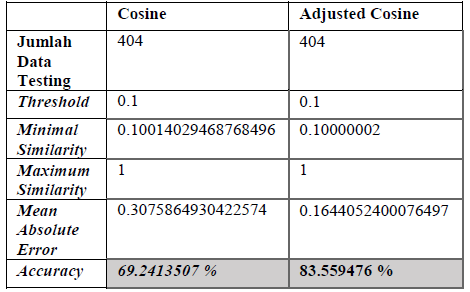
\includegraphics[width=160mm]{gambar/akurasi-algoritma-cosine-similarity.png}
\end{table}

Dan mendapatkan akurasi pada data \emph{testing} menggunakan model \emph{K-Nearest Neighbors} dengan jumlah K = 16 sebesar 89.31\%
dan mendapatkan Mean Absolute Error sekitar 10.75.
\newpage

\begin{figure} [ht] \centering
  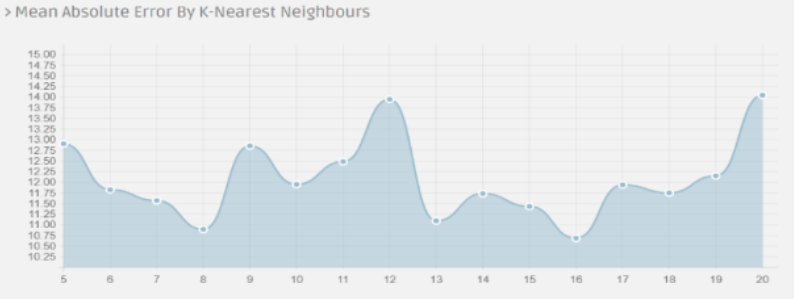
\includegraphics[width=160mm]{gambar/mae-knn.png}
  \vspace*{2mm}
  \caption{Visualisasi Mean Absolute Error model \emph{K-Nearest Neighbors} \citep{cosineSimilarity}}
\end{figure}

Pada tahun 2022 Edward Fernando, Panca Mudjiraharjo, dan Muhammad Aswin melakukan penelitian untuk membuat sistem rekomendasi
dengan pendekatan \emph{Collacorative filtering} dan algoritma \emph{K-Means Clustering}. Dalam penelitian ini, sistem rekomendasi
berbasis collaborative filtering dibangun dengan empat metode, yaitu \emph{jaccard distance}, \emph{euclidean distance}, \emph{cosine similiarity}, dan \emph{pearson correlation}.
Dari pengimplementasian keempat metode tersebut, sistem mampu melakukan prediksi terkait konsentrasi prodi mahasiswa dan juga rekomendasi mata kuliah
yang dapat diambil pada semester selanjutnya. Dari implementasi awal, didapatkan hasil bahwa metode yang paling optimal hingga yang kurang optimal
secara berurutan adalah metode \emph{cosine similiarity}, \emph{euclidean distance}, \emph{jaccard distance}, lalu \emph{pearson correlation}.

\begin{table} [ht] \centering
  \caption{Nilai Kenaikan Akurasi Pendekatan \emph{Collaborative Filtering} dengan \emph{K-Means Clustering} \citep{clustering}}
  \vspace*{2mm}
  \resizebox{\columnwidth}{!}{
    \begin{tabular}{|c|cc|c|}
      \hline
      \multirow{2}{*}{Metode} & \multicolumn{2}{c|}{\begin{tabular}[c]{@{}c@{}}Moving Average Akurasi \\ MK\end{tabular}} & \multirow{2}{*}{Kenaikan Akurasi}                                  \\ \cline{2-3}
                              & \multicolumn{1}{c|}{\begin{tabular}[c]{@{}c@{}}Sebelum \\ K-means\end{tabular}}           & \begin{tabular}[c]{@{}c@{}}Sesusah\\ K-Means\end{tabular} &        \\ \hline
      Jaccard                 & \multicolumn{1}{c|}{51.18\%}                                                              & 53.66\%                                                   & 4.83\% \\ \hline
      Euclidean Distance      & \multicolumn{1}{c|}{56.44\%}                                                              & 62.04\%                                                   & 9.92\% \\ \hline
      Cosine Similiarity      & \multicolumn{1}{c|}{59.25\%}                                                              & 64.76\%                                                   & 9.30\% \\ \hline
      Pearson Correlation     & \multicolumn{1}{c|}{40.83\%}                                                              & 43.71\%                                                   & 7.05\% \\ \hline
    \end{tabular}
  }
\end{table}

Proses optimalisasi hasil rekomendasi mata kuliah pada penelitian ini dilakukan dengan melakukan seleksi rekomendasi berdasarkan tabel keputusan
yang dioleh menggunakan metode \emph{K-Means Clustering}. \emph{K-Means Clustering} mampu melakukan klasterisasi dari seluruh mata kuliah yang muncul dalam rekomendasi
dan memberikan label untuk mana mata kuliah yang direkomendasikan dan tidak direkomendasikan. Pada pengimplementasiannya, tabel keputusan \emph{K-Means Clustering}
mampu meningkatkan nilai akurasi \emph{moving average} pada setiap metode pendekatan \emph{collaborative filtering} dengan persentase peningkatan akurasi secara berurutan
dari yang paling optimal hingga kurang optimal yaitu \emph{euclidean distance} sebesar 9.92\%, \emph{cosine similiarity} sebesar 9.30\%, \emph{pearson correlation} sebesar 7.05\%,
dan \emph{jaccard} sebesar 4.83\%. Secara keseluruhan, sistem rekomendasi mata kuliah ini mampu melakukan prediksi konsentrasi mahasiswa hingga 84.78\% dan akurasi
\emph{moving average} pada prediksi rekomendasi mata kuliah hingga 64.76\% menggunakan data latih yang ditentukan. Dengan nilai \emph{mean absolute error} yang dihasilkan
pada penelitian ini, pendekatan \emph{collaborative filtering} yang paling optimal untuk perekomendasian mata kuliah jatuh pada metode \emph{cosine similiarity}.

\begin{table} [ht] \centering
  \caption{Nilai Mean Absolute Error Akurasi Mata Kuliah \citep{clustering}}
  \vspace*{2mm}
  \resizebox{\columnwidth}{!}{
    \begin{tabular}{|c|cc|c|}
      \hline
      \multirow{2}{*}{Metode} & \multicolumn{2}{c|}{\begin{tabular}[c]{@{}c@{}}Moving Average Akurasi \\ MK\end{tabular}} & \multirow{2}{*}{Kenaikan Akurasi}                                  \\ \cline{2-3}
                              & \multicolumn{1}{c|}{\begin{tabular}[c]{@{}c@{}}Sebelum \\ K-means\end{tabular}}           & \begin{tabular}[c]{@{}c@{}}Sesusah\\ K-Means\end{tabular} &        \\ \hline
      Jaccard                 & \multicolumn{1}{c|}{51.18\%}                                                              & 53.66\%                                                   & 4.83\% \\ \hline
      Euclidean Distance      & \multicolumn{1}{c|}{56.44\%}                                                              & 62.04\%                                                   & 9.92\% \\ \hline
      Cosine Similiarity      & \multicolumn{1}{c|}{59.25\%}                                                              & 64.76\%                                                   & 9.30\% \\ \hline
      Pearson Correlation     & \multicolumn{1}{c|}{40.83\%}                                                              & 43.71\%                                                   & 7.05\% \\ \hline
    \end{tabular}
  }
\end{table}

\section{\emph{Deep Learning}}
\emph{Deep learning} merupakan metode \emph{learning}
yang memanfaatkan \emph{artificial neural network} yang berlapis-lapis(\emph{multi layer}). \emph{Artifical Neural Network} ini dibuat mirip otak manusia, dimana \emph{neuron-neuron} terkoneksi
satu sama lain sehingga membentuk sebuah jaringan \emph{neuron} yang sangat rumit. \emph{Deep Learning} atau \emph{deep structured learning} atau \emph{hirarchial learning} atau \emph{deep neural} merupakan
metode \emph{learning} yang memanfaatkan \emph{multiple non-linier transformation}, \emph{deep learning} dapat dipandang sebagai gabungan \emph{machine learning} dengan \emph{AI (artificial neural network)} \citep{deepLearning}.

\section{Sistem Rekomendasi}
Sistem rekomendasi merupakan suatu sistem yang dapat memberikan informasi dan rekomendasi yang membantu pengguna dalam membuat keputusan berdasarkan data yang telah ada sebelumnya
\citep{clustering}. Sistem rekomendasi akan memberikan rekomendasi yang berbeda kepada setiap pengguna, bukan sekedar memberikan daftar item paling banyak diminati, melainkan memberikan
saran mengenai item-item yang mungkin sesuai untuk pengguna. Artinya, setiap pengguna akan mendapatkan rekomendasi yang berbeda, sesuai dengan profil dan minat
pengguna tersebut \citep{contentBasedXCollaborative}.

Sistem ini tidak merekomendasikan item secara spesifik yang pengguna inginkan. Sistem akan merekomendasikan sejumlah item yang mungkin cocok, jadi jangan heran jika
item yang direkomendasikan oleh sistem terkadang tidak sesuai dengan preferensi pengguna. Pada sistem rekomendasi, keluarannya adalah rekomendasi “top-N”. Sistem akan memberikan sejumlah
rekomendasi peringkat teratas yang cocok dengan pengguna.

Meskipun demikian, penentuan rekomendasi personal mensyaratkan bahwa sistem harus memiliki pengetahuan tentang pengguna. Setiap system rekomendasi harus membuat dan
memaintain suatu model pengguna atau profil pengguna yang, misalnya, memuat informasi mengenai minat atau preferences dari pengguna \citep{contentBasedXCollaborative}.

\section{\emph{Content-based Filtering}}
\emph{Content-based Filtering} adalah jenis sistem pemberi rekomendasi yang mencoba menebak apa yang mungkin disukai pengguna berdasarkan aktivitas pengguna tersebut. \emph{Content-based Filtering}
membuat rekomendasi dengan menggunakan kata kunci dan atribut yang ditetapkan ke objek dalam database (misalnya, item di pasar online) dan mencocokkannya dengan profil pengguna.
Sistem rekomendasi dengan metode \emph{content-based filtering} melakukan proses learning untuk merekomendasikan item yang mirip dengan item sebelumnya
yang disukai atau dipilih oleh pengguna. Kemiripan item dihitung berdasarkan pada fitur-fitur yang ada pada item yang dibandingkan. Oleh karenanya, metode ini tidak bergantung
pada situasi apakah item tersebut merupakan item baru {(yang belum pernah dipilih oleh pengguna manapun)} maupun bukan item baru. Konten yang menjadi obyek \emph{learning} pada
metode ini umumnya adalah informasi fitur mengenai item yang tersedia, namun pada perkembangannya, profil pengguna juga dapat menjadi content yang dipelajari
kemiripannya \citep{contentBasedXCollaborative}.

Sistem akan memilih dan melakukan peringkat item berdasarkan kesamaan profil pengguna dan profil item.Kesamaan antara representasi dari pengguna dan representasi dari
item akan didasarkan pada prinsip kedekatan yang menyatakan bahwa jarak dari dua deskripsi item secara langsung berkaitan dengan kesamaan mereka \citep{rekomendasiTanaman}.
Misalnya, jika pengguna memiliki positif menilai film yang termasuk dalam genre komedi, maka sistem dapat belajar untuk
merekomendasikan film lain dari genre ini \citep{handbook}.


\section{\emph{Collaborative Filtering}}
\emph{Collaborative Filtering} adalah suatu konsep dimana opini dari pengguna lain yang ada digunakan untuk memprediksi item yang mungkin disukai/diminati oleh seorang pengguna \citep{handbook}.
\emph{Collaborative filtering} bekerja dengan membuat suatu \emph{database} yang berisi item \emph{preferences} dari pengguna. Sebagai contoh, pengguna A dicocokkan terhadap data yang ada di \emph{database} untuk menemukan
\emph{neighbor}, yaitu pengguna lain yang memiliki kemiripan \emph{preference} dengan pengguna A. Dari kecocokan yang didapatkan, pengguna A akan diberikan rekomendasi item yang sebelumnya pernah dipilih oleh neighbor dari
pengguna A. \emph{Collaborative filtering} mampu memberikan rekomendasi yang lebih dari sekedar kemiripan item, melainkan dapat memberikan rekomendasi dengan mempelajari selera pengguna dan mencari pengguna yang memiliki selera yang kurang lebih sama \citep{contentBasedXCollaborative}.

Pada implementasi \emph{Collaborative filtering} dalam sistem rekomendasi mata kuliah pilihan, data yang dibandingkan akan disimpan dalam sebuah matriks dua dimensi dimana dimensi dari y atau baris akan menyatakan mahasiswa dan dimensi x atau kolom akan menyatakan mata kuliah
\citep{cosineSimilarity}.

\section{\emph{Hybrid Recommender System}}
\emph{Hybrid recommender system} merupakan sebuah konsep dimana sistem rekomendasi dibangun dengan menggabungkan dua atau lebih pendekatan. Terdapat banyak cara untuk mengombinasikan dua atau lebih pendekatan untuk dapat menghasilkan \emph{hybrid recommender system},
salah satu yang paling mudah untuk diterapkan yaitu dengan menggabungkan hasil rekomendasi item yang diberikan oleh masing-masing pendekatan, dengan begitu kekurangan yang dimiliki oleh masing-masing pendekatan dapat bisa dilengkapi oleh pengekatan yang lainnya.

